Um die Robustheit der im Rahmen dieser Arbeit implementierten MCTS- und PPO-Agenten miteinander zu vergleichen, wurden sie in den in Kapitel \ref{robustheit-szenarien} beschriebenen Szenarien im Spiel gegen einen zufällig spielenden Agenten evaluiert. Die Agenten spielen dabei mit abwechselndem Anzugsrecht gegen einen zufällig spielenden Agenten. Gemessen wird die Gewinnrate der zu untersuchenden Agenten in Abhängigkeit des Ausmaßes der in den Szenarien eingeführten Unsicherheit.

Für jeden untersuchten Unsicherheitsgrad wurden mit dem PPO-Agenten 2000 Spiele durchgeführt. Bei den Untersuchungen mit dem MCTS-Agenten wurden auf Grund des erhöhten Rechenbedarfs und der begrenzten Zeit nur 200 Spiele durchgeführt. Wie in Kapitel \ref{konzept} beschrieben, wird der Gewinnratenverlust als relatives Maß für die Robustheit der Verfahren verwendet. Ein höherer Gewinnratenverlust deutet dabei auf ein weniger robustes Verfahren hin. Die tatsächlich gemessenen Gewinnraten im Spiel gegen den zufällig spielenden Agenten befinden sich im Anhang unter ref{}.

\subsection{Unsicherheit bezüglich Aktionen}

Beim Vergleich der Verfahren hinsichtlich der Robustheit gegenüber Unsicherheiten bezüglich Aktionen wurde die Wahrscheinlichkeit, anstelle des durch den Agenten gewählten Zuges einen zufälligen Zug durchzuführen, in 10-Prozentpunktschritten von 0 \% bis 100 \% variiert.

\begin{figure}[ht!]%[!tbp]
	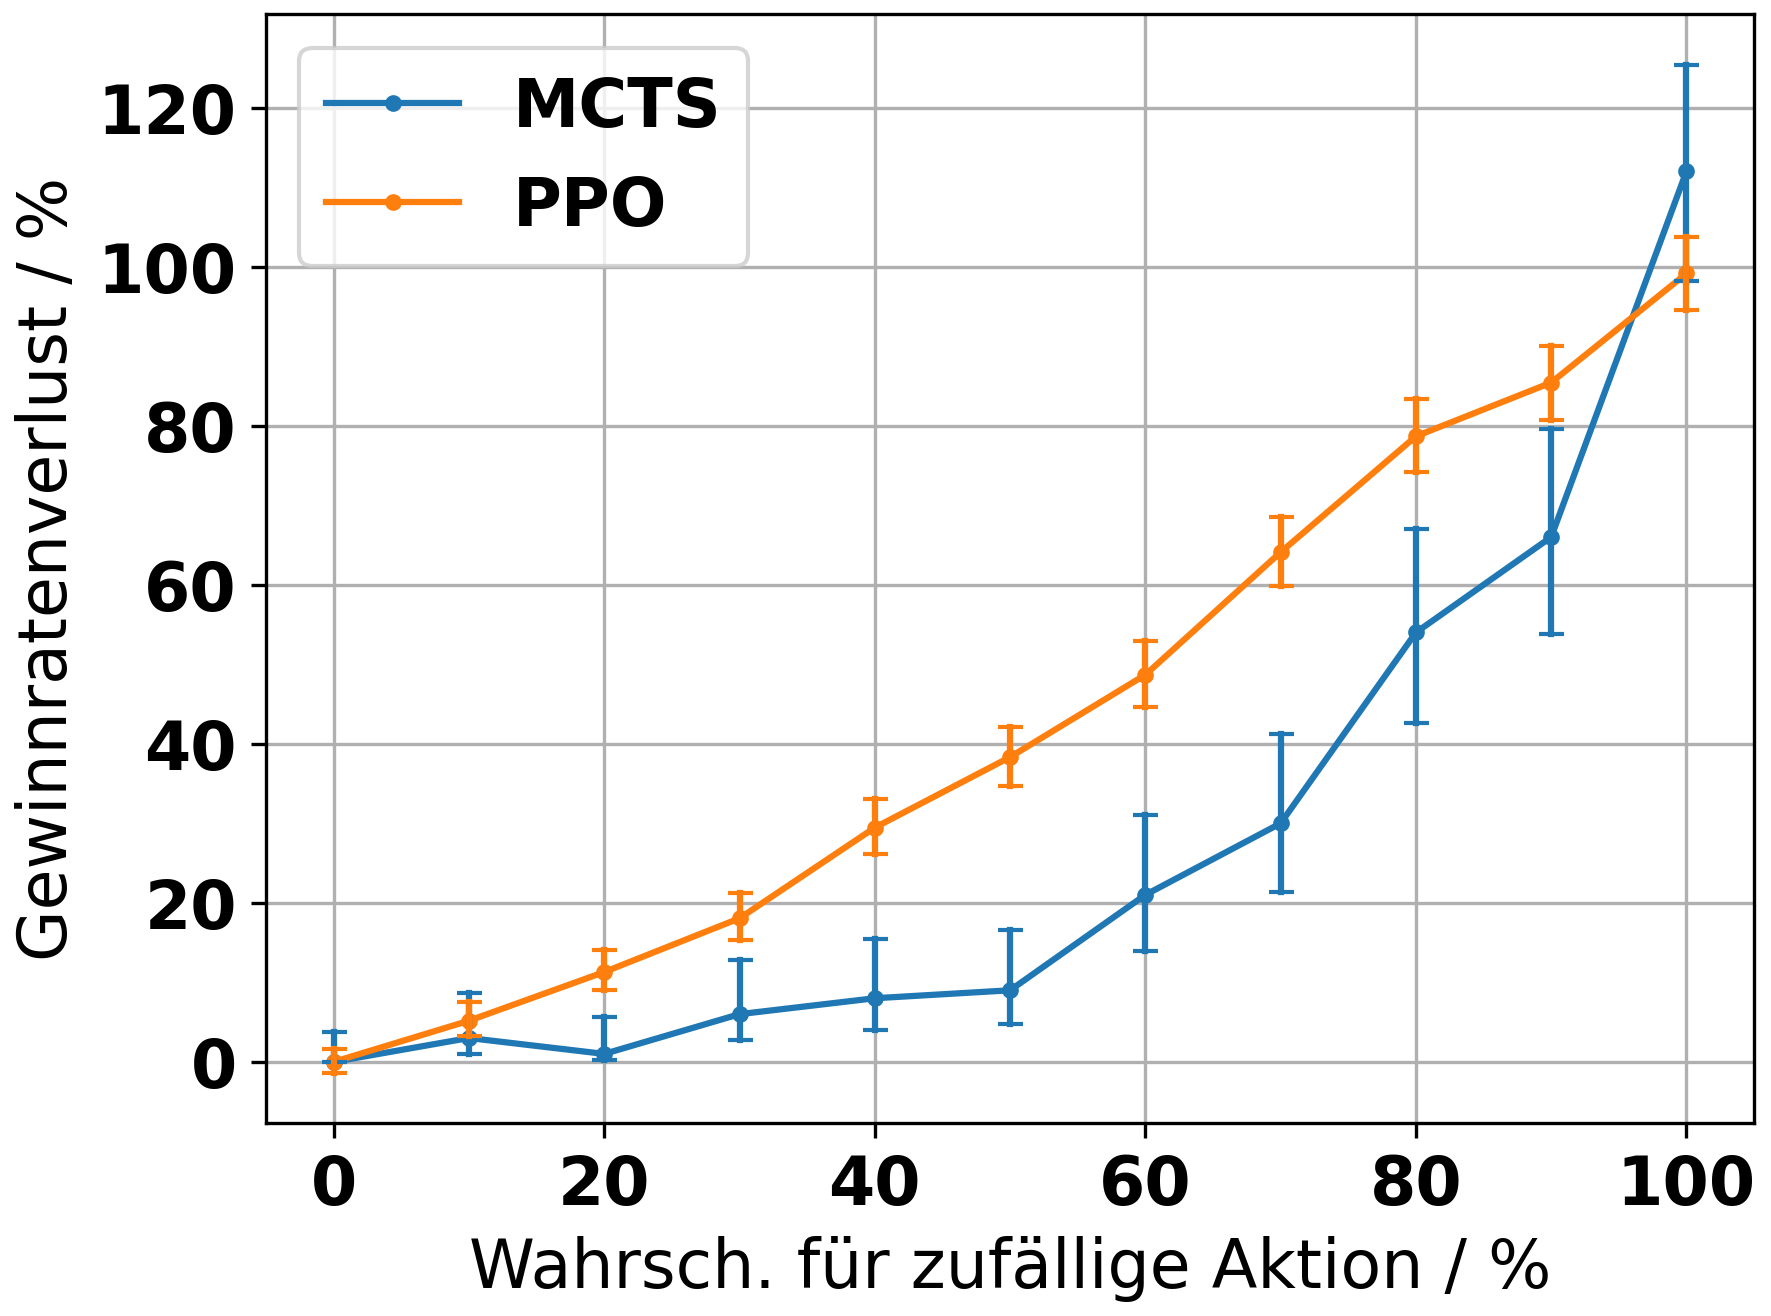
\includegraphics[width=0.7\textwidth, center]{Bilder/robustness-results/uncertain_actions_win_rate_losses.png}
	\caption{Gewinnratenverlust in Abhängigkeit von der Wahrscheinlichkeit, eine zufällige Aktion durchzuführen.}
\end{figure}

Beträgt diese Wahrscheinlichkeit 0 \%, befindet sich der Gewinnratenverlust bei beiden Agenten ebenfalls bei 0 \%, da es sich bei den dabei erzielten Gewinnraten um den Ausgangswert für die Berechnung des Gewinnratenverlustes handelt.

Ab einer Wahrscheinlichkeit für zufällige Aktionen von 20 \% ist für den MCTS-Agenten ein signifikant niedrigerer Verlust von … gegenüber von … bei PPO zu verzeichnen. Einen solche signifikante Differenz hält sich bis zu einer Wahrscheinlichkeit von 80 \% für zufällige Aktionen, wo ein Gewinnratenverlust von … beim MCTS-Agenten und … beim PPO-Agenten ermittelt wurde. Damit ist der MCTS-Agent in diesem Bereich signifikant robuster als der PPO-Agent.

Bei 90 \% liegen die Messpunkte von MCTS zwar mit … gegenüber … zwar weiterhin höher, aber die Konfidenzintervalle der Messpunkte sind so nah bei einander, dass aus den Werten allein nicht mit ausreichender Sicherheit Schlüsse über die tatsächlichen Werte gezogen werden können.

Bei einer Wahrscheinlichkeit für zufällige Aktionen von 100 \% sollten beide Agenten nach genügend durchgeführten Spielen gegen den zufällig spielenden Agenten eine Gewinnrate von 50 \% und damit einen Gewinnratenverlust von 100 \% erzielen. Die Messpunkte liegen für MCTS mit … leicht darüber bzw. für PPO mit … leicht darunter. Da ein Gewinnratenverlust von 100 \% innerhalb der Konfidenzintervalle liegt, ist es naheliegend, dass die gemessenen Abweichungen stochastisch bedingt sind.

Aus den Messungen geht für eine Wahrscheinlichkeit für zufällige Aktionen von 20 \% bis 80 \% der MCTS-Agent als der robustere Agent hervor. Für darunter bzw. darüber liegende Wahrscheinlichkeiten kann aufgrund von Messungenauigkeiten kein signifikanter Unterschied festgestellt werden. Der Verlauf des Gewinnratenverlusts liegt jedoch nahe, dass MCTS auch dort weiterhin einen niedrigen tatsächlichen Verlust aufweist.

Es wurde nicht erwartet, im Szenario mit Unsicherheiten bezüglich Aktionen eine signifikante Differenz im Gewinnratenverlust zwischen den beiden Verfahren zu sehen, die durch die Verfahren selbst bedingt sind. Es liegt nahe, dass die Diskrepanz dadurch hervorgerufen wird, dass der PPO-Agent unzureichend trainiert wurde, wodurch er eine kurzfristigere Strategie besitzt, die anfälliger für Störungen ist. Daher können aus den Messungergebnissen keine Schlüsse darüber gezogen werden, welches der beiden Verfahren grundsätzlich robuster gegenüber Unsicherheit bezüglich Aktionen ist. Somit sind in dieser Hinsicht auch keine verallgemeinernden Aussagen über symbolische Algorithmen und Reinforement Leraning möglich.

\subsection{Unsicherheit bezüglich Beobachtungen}

Beim Vergleich der Verfahren hinsichtlich der Robustheit gegenüber Unsicherheiten bezüglich Beobachtungen wurde die Anzahl von fehlerhaften Spielsteinplatzierungen, in 2er-Schritten von 0 bis 20 variiert. Aufgrund der größer werdenden Konfidenzintervalle wurden ab 10 fehlefhaften Spielsteinplatzierungen nicht mit 200 sondern 500 Spiele zwischen dem MCTS-Agenten und dem zufällig spielenden Agenten ausgetragen.

\begin{figure}[ht!]%[!tbp]
	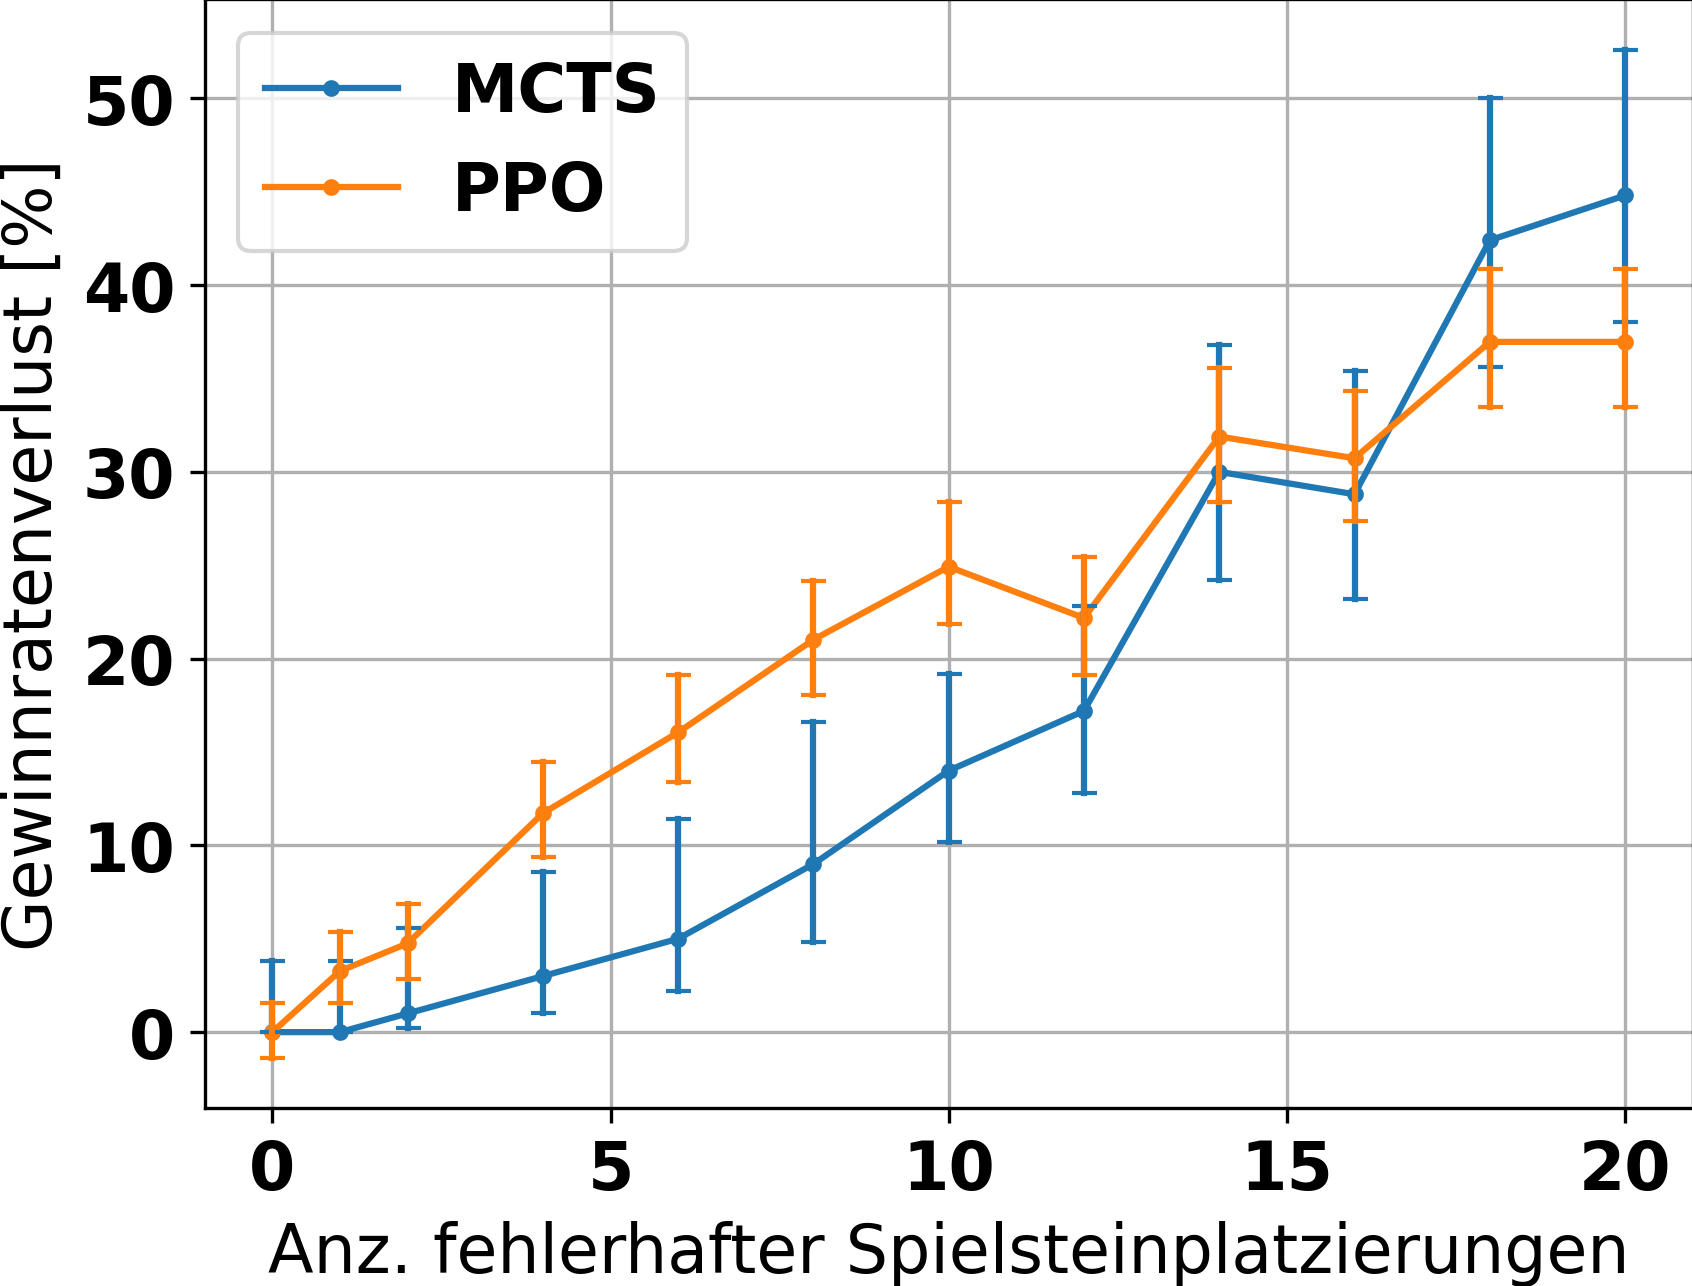
\includegraphics[width=0.7\textwidth, center]{Bilder/robustness-results/uncertain_observations_win_rate_losses.png}
	\caption{Gewinnratenverlust in Abhängigkeit von der Anzahl fehlerhafter Spielfeldplatzierungen.}
\end{figure}

Ähnlich wie in … startet der Gewinnratenverlust beider Agenten bei 0 fehlerhaften Spielsteinplatzierungen mit 0 \%.

Ab 4 fehlerhaften Spielsteinplatzierungen lässt sich bei MCTS mit … ein signifikant niedrigerer Gewinnratenverlust gegenüber PPO mit … verzeichnen. Diese Diskrepanz hält sich bis zu einer Anzahl von 10 fehlerhaften Platzierungen, wobei der MCTS-Agent einen Gewinnratenverlust von … und der PPO-Agent einen Verlust von … erzielt. Das zeigt, dass sich der MCTS-Agent in diesem Bereich signifikant robuster verhält als der PPO-Agent.

Ab 12 fehlerhaften Platzierungen sind die Differenzen zwischen den Messpunkten zu niedrig und die Konfidenzintervalle so groß, dass nicht mit ausreichender Sicherheit bestimmt werden kann, bei welchem Agenten die tatsächlichen Werte höher oder niedriger liegen.

Bei 18 und 20 fehlerhaft platzierten Steine liegt der gemessene Verlust von MCTS mit … und sogar über dem von PPO mit … und …, aufgrund der großen Konfidenzintervalle kann jedoch nicht gesagt werden, ob sich die tatsächlichen Werte genauso verhalten. Um Aussagen darüber treffen zu können, sind Messungen mit mehr Wiederholungen nötig.

Bei 4 bis 10 fehlerhaften Spielsteinplatzierungen geht der MCTS-Agent als der robustere Agent hervor. Aufgrund des Verlaufs des Gewinnratenverlusts in Abhängigkeit er fehlerhaften Spielsteinplatzierungen liegt nahe, dass dies auch für unter einer Anzahl von 4 gilt. Liegt die Anzahl der fehlerhaften Spielsteinpkatzierungen über 10 können aufgrund der zu großen Messungenauigkeiten keine signifikanten Unterschiede festgestellt werden. Die beobachtete höhere Robustheit des MCTS-Agenten könnte durch die Anfälligkeit von neuronalen Netzwerken gegenüber unerwarteten Beobachtungen verursacht worden sein. Ebenso wie in … könnte die Ursache für dieses Verhalten jedoch auch in der kurzfristigen Strategie des in dieser Arbeit unzureichend trainierten PPO-Modells liegen. Damit können auch hier keine Aussagen darüber getroffen werden, welches der beiden Verfahren MCTS oder PPO bzw. symbolischer Algorithmus oder Reinforcement Learning grundsätzlich robuster gegenüber Unsicherheiten bezüglich Beobachtungen ist.

Auch wenn aufgrund des unzureichenden Trainings des in der Arbeit implementierten PPO-Agenten keine Aussagen getroffen werden können, die auf die Verfahren verallgemeinert werden können, ist anzumerken, keine Überraschung in der Hinsicht aufgetreten ist, als dass der PPO-Agent trotz seiner unterlegenen Strategie als signifikant robuster gemessen wurde als der MCTS-Agent.

Um Aussagen über das Verhalten der Agenten auf die Verfahren MCTS und PPO bzw. symbolischer Algorithmus und Reinforcement Learning verallgemeinern zu können, muss sichergestellt sein, dass die Agenten unter neutralen Bedingungen möglichst die selbe Leistung erzielen. Im Rahmen dieser Arbeit konnten durch quantitative und qualitative Analysen der Agenten gezeigt werden, dass dies in diesem Fall nicht zutrifft. Es ist kritisch zu hinterfragen, inwiefern diese Methodiken ausreichen würden, um zu zeigen, dass die Agenten dieselbe Leistung erzielen. Denn im Spiel gegen einen zufällig spielenden Agenten spiegeln sich große Leistungsunterschiede nur in sehr kleinen Differenzen wieder. Und in der qualitativen Analyse können subjektive Verzerrungen der Wahrnehmung das Ergebnis beeinflussen. Besser geeignet sind beispielsweise das Spiel gegen einen perfekt spielenden Agenten wie in … oder gegen unterschiedliche nicht-perfekt spielende Agenten in einer Turnier-Umgebung, so wie es in … umgesetzt wurde.



